\chapter{Infraestructura}
\label{cap:infra}

En este Capítulo describiremos la infraestructura utilizada, tanto software como hardware, detallando los pasos a seguir si se desea reproducir. En caso de que algún componente haya sido elegido entre otros de igual aplicación, expondremos las razones de la elección.


\section{Entorno}\label{sec:entorno}
Teniendo el cuenta el carácter educativo de este Trabajo, y su pretendida aplicación en estudiantes de Educación Primaria, se ha elegido el sistema operativo Windows, un entorno conocido, amigable y fácilmente accesible, para instalar y utilizar las diferentes herramientas software. \\
Tradicionalmente, cuando se hablaba de programación y especialmente de programación robótica, siempre se ha utilizado el sistema operativo Linux. Éste daba la posibilidad de instalar todos los paquetes de lenguajes de programación y entornos, mientras que Windows era especialmente cerrado en cuanto a lenguajes no nativos (fuera de \textit{bash} o de \textit{visual basic}, se hacía complicado utilizar un lenguaje de programación sin acabar recurriendo a virtualizar una máquina Linux), y los entornos software (aplicaciones) de terceros diseñados para programar habitualmente no tenían una versión instalable para Windows. \\
Sin embargo, los últimos años el Sistema Operativo se ha abierto a esta operativa, ya que la política popular demandaba poder utilizarlo como herramienta de desarrollo también a nivel usuario. La nueva línea de comandos de Windows, \textit{\textit{Powershell}} (también lenguaje de scripting) añadió a la original \textit{Bash} características nativas de Linux, siendo una herramienta de programación además de administración. De hecho, en la última versión, está disponible para el propio SO de Linux (en algunas distribuciones). \\
Al principio de este Trabajo, se consideró a Linux un entorno menos amigable para usuarios sin experiencia en programación por ser considerado ``no de usuario". En el poco probable caso de que un estudiante conociera el sistema, lo consideraba algo muy complejo y no accesible para su nivel. Por tanto, elegir Windows eliminaba ese prejuicio y contaba con la ventaja de predisponer positivamente al alumno y de facilitarle el acceso al entorno. 

\section{Hardware}\label{sec:hardware}
En esta sección describiremos los componentes hardware utilizados. La razón de la elección de éstos responde a la misma filosofía de facilitar el acceso a los componentes y la facilidad con que éstos se complementan en el entorno.
\subsection{Placa Arduino}\label{subsec:placaBase}
Las placas Arduino son las más extendidas en cuanto a robótica. El proyecto de Arduino \cite{arduinoURL} nació como una solución barata con el principal objetivo de utilizar sus componentes y recursos en Educación. Al ser un proyecto liberado al público, su uso está extendido a toda una comunidad, que amplía y comparte sus propios desarrollos.\\
Estas placas base son hardware libre, uno de las principales razones de su bajo coste. Contienen un procesador re-programable y una serie de pines hembra, donde se conectarán los periféricos de entrada/salida necesarios para controlar un robot. Hay diferentes modelos de placas Arduino, cada una fabricada con un propósito diferente. En este caso, hemos utilizado el modelo mCore, basado en Arduino Uno\footnote{\href{https://arduino.cl/producto/arduino-uno/}{https://arduino.cl/producto/arduino-uno/}}, ya que es la que lleva por defecto el robot educativo mBot (que comentaremos en la sección \ref{subsec:mbot}). Además de los pines hembra, o puertos, contiene una serie de actuadores y sensores integrados en la placa.
\begin{figure}[H]
		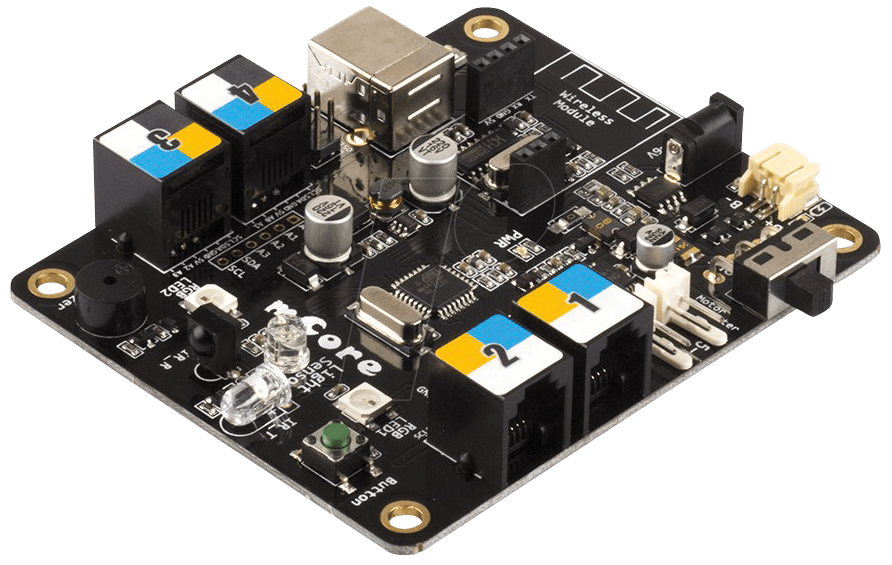
\includegraphics[width=8cm]{mcore.png}\centering
	\label{img:Mcore}
	\caption{Placa mCore}
\end{figure}
\subsection{mBot}\label{subsec:mbot}
Actualmente hay una gran variedad de robots educativos, orientados principalmente a los alumnos más jóvenes. El objetivo de la robótica educativa es ofrecer un entorno amigable, divertido y más \textit{realista} que la programación tradicional. Es más fácil para un niño o niña sentirse interesado por algo que tiene una reacción \textit{visible}, en algo que puede tocar y manejar, que en la programación normal que produce una reacción mucho más abstracta. Esto convierte la robótica en la herramienta perfecta para enseñar lenguajes y conceptos básicos de programación (como funciones o uso de variables) y con el que avanzar hasta la algoritmia se hace un proceso natural al que los propios alumnos llegan ellos mismos. \\

El principal problema al que nos enfrentamos para enseñar programación a los más jóvenes son los lenguajes de programación. Son poco intuitivos y legibles, a lo que se suma la dificultad de mantener la atención de un alumno o alumna tan joven escribiendo en un ordenador durante mucho tiempo. Era necesaria, por tanto, una forma de enseñar los conceptos de programación comentados sin tener que utilizar lenguajes clásicos de programación, al menos para los alumnos más jóvenes. La solución fue la programación por bloques de \textit{pseudocódigo}. El pseudocódigo es un \textit{framework}, una carcasa, que recubre el verdadero lenguaje de programación de la placa del robot y lo hace legible y entendible. Además, una de las grandes ventajas añadidas es que la mayoría de los pseudocódigos están en casi todos los idiomas, permitiendo a los alumnos programar en su propio idioma. \\
\par Esto nos lleva al robot mBot del fabricante Makeblock \cite{makeblock}. Está basado en una placa Arduino Uno y pensado especialmente para la enseñanza. Los diferentes sensores y actuadores (los que vienen en el paquete básico, aunque hay muchos más posibles del mismo fabricante) están pensados para ofrecer ejercicios entretenidos y, lo más importante, con diferentes niveles de dificultad. Esto lo hace perfecto para ser utilizado con alumnos de diferentes edades y crear prácticas con las que evolucionar en los conceptos. 
\begin{figure}[H]
	\includegraphics[width=8cm]{Mbot.jpg}\centering
	\caption{Modelo mBot utilizado}
	\label{img:mbot}
\end{figure}
Este robot mBot puede programarse utilizando un  lenguaje llamado \textit{Scratch},  un pseudocódigo muy gráfico y sencillo pero potente, que ``recubre'' la placa base. Sin embargo, al ser las placas Arduino reprogramables, siempre se puede programar en el propio lenguaje Arduino. Esto  se explicará en profundidad más adelante, en el Capítulo \ref{cap:PyBoKids}. \\

Como puede observarse en la figura \ref{img:mbot}, el robot cuenta con dos motores conectados a la placa; contiene además cuatro puertos numerados a los que poder añadir diferentes periféricos con los que trabajar. Aunque el modelo mostrado es el básico, se pueden cambiar los componentes añadiendo y/o cambiando la estructura base y crear ``otro'' robot (por ejemplo, en las imágenes de la figura \ref{img:mbot2} ). Aunque en este Trabajo de Fin de Grado solo trabajaremos con la versión básica del mBot, esta posibilidad de añadirle componentes o cambiarlos es muy interesante para los alumnos, ya que trabajan la mecánica y pueden utilizar más tipos de periféricos.
\begin{figure}[H]
	\includegraphics[width=6cm]{Mbot-pack-piernas.jpg}
	\includegraphics[width=6cm]{Mbot-pack-piernas2.jpg}
	\centering
	\caption{Posibles cambios en el mBot}
	\label{img:mbot2}
\end{figure}
\subsubsection{Sensores}\label{ssubsec:sensores}
En robótica un \textit{sensor} es un periférico de entrada que, conectado a una placa base, recoge información del medio (cantidad de ruido, temperatura, distancia frontal, etc) y la envía a la placa, dejándola disponible para toma de decisiones. La cantidad de información que se pueda recibir sólo depende de la cantidad de sensores que se pueda conectar a la vez a la placa (cuatro, en este caso, si solo se trabajara con sensores y ningún actuador). En el robot básico (de la figura \ref{img:mbot}) los sensores son los siguientes:
\begin{description}
	\item [Sensor de ultrasonidos] Está colocado en el frente, y recoge información de \textit{distancia} hasta un objeto medida en \textit{cm} (el valor máximo es 400). Puede verse en la figura \ref{img:ultrasonidos}
	
	\item [Sensor infrarrojo \textit{Sigue Líneas}] Se compone en realidad de dos sensores, izquierdo y derecho, por lo que habrá cuatro posibilidades de respuesta del sensor completo. Cada uno de los sensores lee de forma binaria si está sobre tapado o no. A cada posibilidad le corresponde un valor numérico (el valor que devuelve el sensor a la placa Arduino):
	\begin{itemize}
		\item Ningún sensor tapado: 0
		\item Sensor izquierdo tapado y derecho no: 1
		\item Sensor derecho tapado e izquierdo no: 2
		\item Los dos sensores tapados: 3
	\end{itemize}
	Por defecto, está ubicado de tal forma que lea del ``suelo'' si el sensor está tapado o no, de ahí el nombre de \textit{sigue líneas}. Este sensor puede verse en la figura \ref{img:siguelineas}
	
	\item [Sensor de Luz] En este caso, está integrado en la placa (podemos verlo en la figura \ref{img:sensorluz}), por lo que no es necesario utilizar un puerto para él. Nos da un valor de cantidad de luz en el ambiente, pudiéndolo utilizar para saber si hay más o menos luminosidad de la deseada. Por supuesto, para este valor de luz ``deseado'' será necesario obtener un valor inicial de la habitación en la que nos encontremos, con el que establecemos ese valor umbral.
\end{description}
\begin{figure}[H]
	\begin{center}
		\begin{subfigure}
			[Ultrasonidos: sensor de distancia]{
			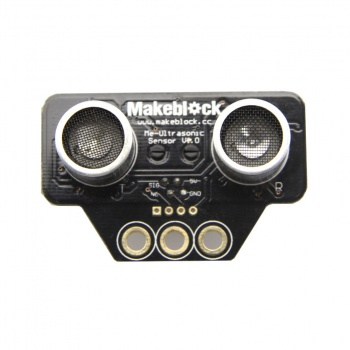
\includegraphics[width=0.45\textwidth]{ultrasonidos.jpg}
			\label{img:ultrasonidos}}
		\end{subfigure}
		\begin{subfigure}
			[Infrarrojos: sensor siguelíneas]{			
			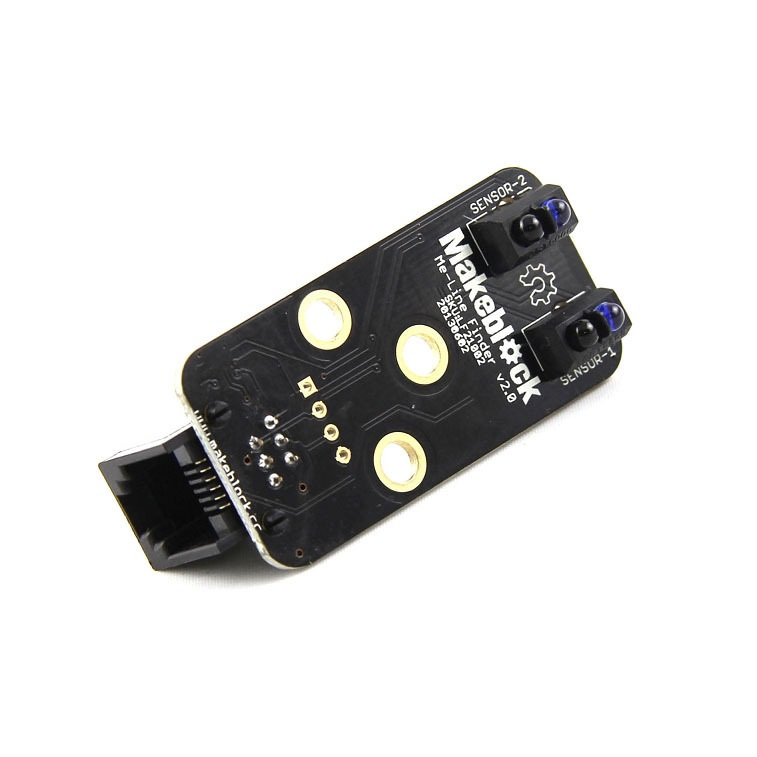
\includegraphics[width=0.45\textwidth]{siguelineas.jpg}
			\label{img:siguelineas}}
		\end{subfigure}
		\begin{subfigure}
			[Sensor de luz integrado]{			
			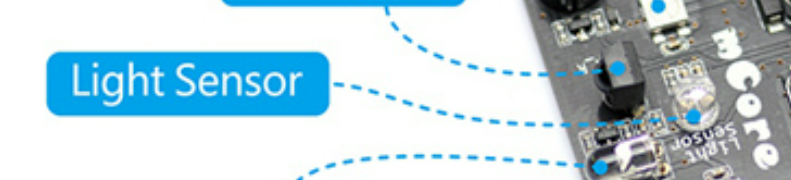
\includegraphics[width=0.45\textwidth]{sensorLuz.png}
			\label{img:sensorluz}}
		\end{subfigure}
	
	\caption{Sensores del mBot}
	\label{img:sensores}
	\end{center}
\end{figure}


\subsubsection{Actuadores}\label{subsec:actuadores}
	La definición de \textit{actuador} es un periférico de salida al que la placa envía datos con los que éste realiza una acción de una forma u otra. Por ejemplo, teniendo una velocidad $v_0$, este valor es enviado a los motores, que se moverán a esa velocidad y no a otra. \\
	Los actuadores del mBot que no están integrados en la placa directamente, se conectan a ella a través de los mismos puertos que los sensores. Para poder usarlos, habrá que especificarle a la placa en qué puerto están conectados (igual que con los sensores). En nuestro robot básico tenemos los siguientes actuadores:
	\begin{description}
	\item [LEDs]. Están integrados en la parte superior de la placa, como puede verse en la figura \ref{img:LED}. Son dos LED individuales que poder combinar dependiendo de qué valor codificado se envíe a la placa:
	\begin{itemize}
		\item Los dos LED: 0
		\item Sólo LED derecho: 1
		\item Sólo LED izquierdo: 2
	\end{itemize}
	Los LED son RGB (\textit{[red, green, blue]}) y el color de cada uno se codifica con un valor numérico entre 0 y 255 para cada uno de los colores (rojo, verde y azul). Así, por ejemplo, el rojo completo sería [0,255,0], el morado sería [255,0,255] o el blanco [255,255,255]. Estos LED están codificados con valores decimales en vez de hexadecimales como sería una codificación RGB tradicional, para facilitar la programación a los alumnos (no es probable que conozcan el sistema hexadecimal).		
	
	\item [Motores] En el paquete básico tenemos dos motores DC (de corriente continua) conectados a la placa en un conector específico para motores a los que conectar los dos cables, positivo y negativo. Los motores admiten como velocidad de entrada valores enteros entre [-255,255] (valores negativos para retroceder y positivos para avanzar), pudiendo dar valores diferentes a cada uno de ellos (para tener capacidad de hacer girar al robot). En la figura \ref{img:motores} se puede ver un ejemplo del motor y de la forma de conectarlo al mBot.	

	\item [Zumbador] También está integrado en la placa, como puede verse en la figura \ref{img:zumbador}. Emite notas musicales, codificadas en Scratch con nomenclatura americana. La equivalencia con la nomenclatura europea, que los alumnos necesitan conocer, está en la tabla \ref{table:notasZumbador}. Para utilizar notas más agudas o más graves, se utilizan números a continuación de las letras (Por ejemplo, \textit{C0} es más grave que \textit{C5}). Internamente (si programáramos el robot con Arduino) el zumbador entiende valores enteros, correspondientes en frecuencia con cada nota (en la tabla sólo se pone un valor para cada nota a modo de ejemplo):
	\begin{table}[h]
		\centering
		\begin{tabular}{ c | c | c}	
			Europea & Americana & Valor entero \\
			\hline			
			Do & C & 33\\
			RE & D & 37\\
			MI & E & 41\\
			FA & F & 44\\
			SOL & G & 49\\
			LA & A & 55\\
			SI & B & 62\\
		\end{tabular}
	
	\caption{Relación entre notas para el Zumbador del mBot}
	\label{table:notasZumbador}
	\end{table}	
\end{description}

\begin{figure}[H]
	\includegraphics[width=3cm]{RGBled.png}
	\centering
	\caption{LED RGB integrados}
	\label{img:LED}
\end{figure}

\begin{figure}[H]
	\begin{center}
		\begin{subfigure}
			[Puerto de conexión de los motores]{
				\includegraphics[width=0.45\textwidth]{puertomotor.png}
				\label{img:puertomotor}}
		\end{subfigure}
		\begin{subfigure}
			[Motor DC]{			
				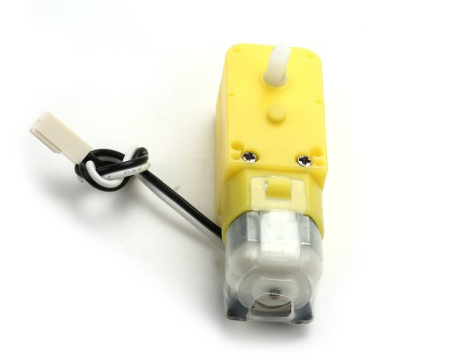
\includegraphics[width=0.33\textwidth]{motorDC2.png}
				\label{img:motor1}}
		\end{subfigure}
		\begin{subfigure}
			[Motor DC: montaje con rueda]{			
				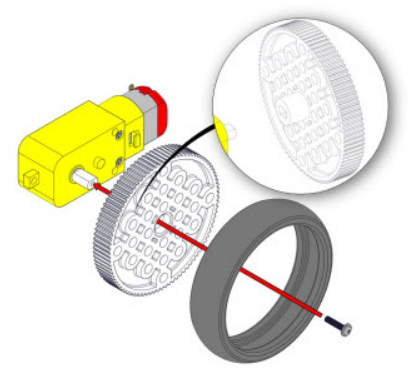
\includegraphics[width=0.33\textwidth]{motorDC.png}
				\label{img:motor2}}
		\end{subfigure}				
		\caption{Motores}
		\label{img:motores}
	\end{center}
\end{figure}

\begin{figure}[H]
	\includegraphics[width=3cm]{buzzer.png}
	\centering
	\caption{Zumbador integrado}
	\label{img:zumbador}
\end{figure}

\section{Software}\label{sec:software}
En esta sección describiremos el diferente software utilizado y el propósito de éste en el marco de este Trabajo Fin de Grado. 

\subsection{Scratch y mBlock}\label{subsec:scratch}
Como se ha comentado anteriormente, el robot mBot es programable con Scratch, un lenguaje de programación por bloques. Un \textit{bloque de código} consiste en codificar en un ``paquete'' una sentencia completa de lenguaje (del lenguaje correspondiente, Arduino en este caso). Así, el estudiante que utilice Scratch, será capaz de utilizar una sentencia \textit{if..else} o un bucle \textit{for} de forma muy fácil y entendible, sin necesitar aprenderse todas las reglas de sintaxis del lenguaje real. En la figura \ref{img:scratch}, se muestran algunos ejemplos de bloques en Scratch correspondientes a los conceptos de programación más utilizados.
\begin{figure}[H]
	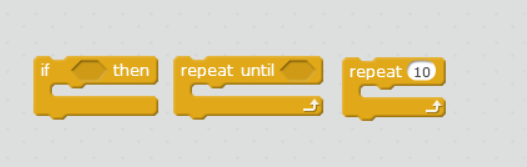
\includegraphics[]{scratch.png}
	\centering
	\caption{Algunos ejemplos de bloques en Scratch}
	\label{img:scratch}
\end{figure}
Las sentencias que se quieran repetir, o las variables de condición, tienen un lugar muy intuitivo donde colocarse. Además, pueden crearse variables, en las que guardar los valores de los sensores y poder utilizar como entrada de actuadores, o como valores de referencia. \\
Scratch puede utilizarse como lenguaje de programación ``tradicional'' (sin robot físico), utilizando un escenario virtual con un personaje para observar el resultado del programa, pero es mucho más completo al añadirle el módulo del robot deseado. Este módulo contiene bloques para recoger valores de los sensores o enviarlos a los actuadores, ya sean \textit{on board} (integrados en la placa) o teniendo que especificar el puerto al que están conectados:
\begin{figure}[H]
	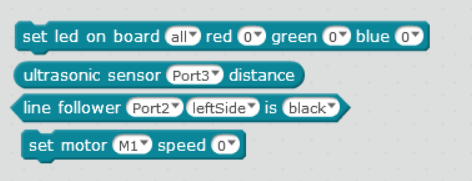
\includegraphics[]{scratch2.png}
	\centering
	\label{img:scratch2}
	\caption{Ejemplos de bloques de mBot en Scratch}
\end{figure}

Para utilizar Scratch y programar el robot es necesario instalar un programa llamado \textit{mBlock}, que es el que contiene el compilador y el que permite conectar el robot al PC para enviarle el programa. El ejecutable se descarga de la página oficial del fabricante\footnote{\href{https://www.makeblock.es/blog/descargas/}{https://www.makeblock.es/blog/descargas/}}, Makeblock, disponible para PC (también existe una versión simplificada para dispositivos móviles).\\
\begin{figure}[h]
	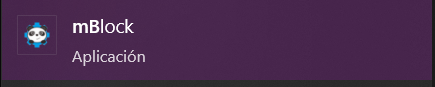
\includegraphics[]{mblockApp.png}
	\centering
	\caption{mBlock en Windows}
	\label{img:mblockApp}
\end{figure}
Una vez instalado el software en nuestro pc (en la figura \ref{img:mblockApp}), el proceso para poder empezar a usar el mBot es muy simple:
\begin{enumerate}\label{list:conexionMblock}
	\item Conectar el robot al pc con el cable USB, y conectarlo con el programa (el robot debe estar encendido):
	\begin{figure}[H]
		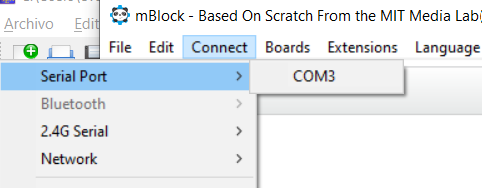
\includegraphics[]{mblock.png}
		\centering
		\label{img:mblock}
		\caption{Conectar el mBot}
	\end{figure}

	\item  Asegurarse de que la placa corresponde con el robot que tenemos:
	\begin{figure}[H]
		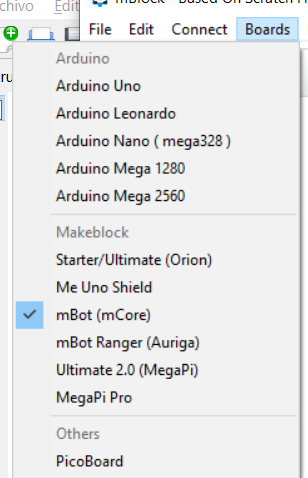
\includegraphics[]{mblock2.png}
		\centering
		\label{img:mblock2}
		\caption{Placa mBot}
	\end{figure}

	\item Actualizar el programa Arduino subido a la placa base, para que funcione con Scratch (en caso de haber utilizado el robot con otro programa):
	\begin{figure}[H]
		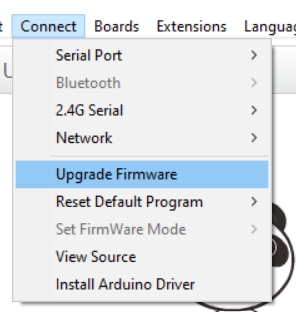
\includegraphics[]{mblock3.png}
		\centering
		\label{img:mblock3}
		\caption{Actualizar firmware de la placa}
	\end{figure}

	\item Para subir código al robot:
		\begin{itemize}
			\item Click derecho sobre el código (figura \ref{img:uploadArduino1}) y click en 'upload to Arduino'. Esto transforma el programa de Scratch a lenguaje Arduino.
			\item Cuando el compilador aparezca en la parte derecha de la pantalla, pulsar en 'upload to arduino' para subirlo a la placa (figura \ref{img:uploadArduino2})
		\end{itemize}
	\begin{figure}[H]
		\centering
		\begin{subfigure}
			[Compilar programa]{
				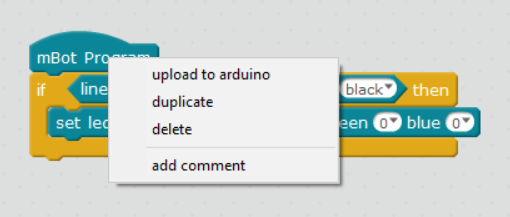
\includegraphics[width=0.45\textwidth]{mblock4.png}
				\label{img:uploadArduino1}}
		\end{subfigure}
		\begin{subfigure}
			[Subir programa a la placa]{
				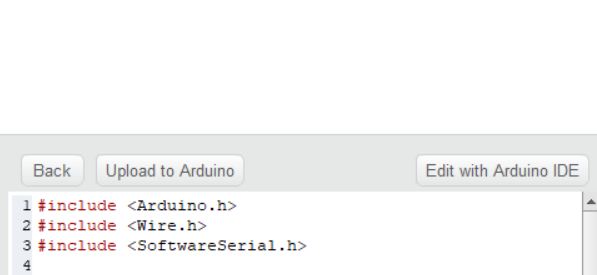
\includegraphics[width=0.5\textwidth]{mblock5.png}
				\label{img:uploadArduino2}}
		\end{subfigure}
	\caption{Subir programa a la placa del mBot}
	\label{img:uploadArduino}
	\end{figure}

	\item Una vez subido el programa, el robot comenzará a funcionar tal y como lo hayamos programado.
\end{enumerate}
 

\par Este lenguaje y la interfaz gráfica, funcionan como una perfecta primera aproximación a la programación y a la robótica, dando más importancia al aprendizaje conceptual que a la sintaxis y al lenguaje. \\
Obviamente, los alumnos necesitarán que se les guíe en comprender las necesidades de incluir los diferentes bloques y las ventajas que éstos producen en el código, sobre todo al comienzo del curso. El objetivo no será explicarles para qué usar, por ejemplo, un bloque condicional, sino proponer un ejercicio cuya solución necesite un condicional, para que lleguen por ellos mismos a la necesidad de usarlo.
\subsection{Arduino}\label{subsec:arduino}
Como se explicó en la sección \ref{subsec:placaBase}, la placa base del robot mBot se programa en \textit{Arduino}\cite{arduinolenguaje}. Este lenguaje de programación está basado en C++ y pensado para interactuar con objetos electrónicos. \\
Para programar el robot mBot en Python primero debe \textit{entender} esas órdenes programadas en Python. Para crear este ``framework'' se utiliza el lenguaje nativo de la placa base, por lo que es necesario instalar el entorno Arduino. Las instrucciones para instalar este entorno en Windows y configurarlo para el robot se detallan a continuación:
\begin{enumerate}\label{list:InstalacionArduino}
	\item Descargar e instalar Arduino IDE, el cual instala el entorno completo de Arduino. Para las versiones 8 y 10 de Windows, está disponible directamente en el Microsoft Store. Para otras versiones de Windows, está disponible en la página web oficial\footnote{\href{https://www.arduino.cc/en/software}{https://www.arduino.cc/en/software}}.
	\begin{figure}[h]
		\includegraphics[width=10cm]{store.png}
		\centering
		\caption{Arduino IDE en el Microsoft Store}
		\label{img:MStore}
	\end{figure}
	\item Descargar las librerías de Makeblock\footnote{\href{https://codeload.github.com/Makeblock-official/Makeblock-Libraries/zip/master}{https://codeload.github.com/Makeblock-official/Makeblock-Libraries/zip/master}} o del siguiente repositorio\footnote{\href{https://github.com/JdeRobot/PyBoKids}{https://github.com/JdeRobot/PyBoKids}} para añadirlas a Arduino y poder utilizarlas en nuestro entorno.
	\item Incluir el archivo comprimido descargado desde el Arduino IDE:\\ \textit{Programa - Incluir librería - Añadir biblioteca .ZIP - Seleccionar el fichero - Abrir}
	\item Seleccionar la placa básica que se va a conectar al IDE:\\
	\textit{Herramientas - Placa - Seleccionar Arduino Uno}
	\item Especificar el modelo exacto de placa al principio del programa de Arduino; en este caso la placa es la mCore. Así se cargan todos los métodos correspondientes al modelo de placa; debe incluirse en cada programa de Arduino que se escriba.
	\begin{verbatim}	
				#include "MeMCore.h"	
	\end{verbatim}
	\item Igual que con Scratch, primero se debe conectar el robot al software (con el robot enchufado al PC y encendido):\\
	\textit{Herramientas - Puerto - Seleccionar el puerto en el que está el robot} \\
	Los puertos USB en Windows son \textit{COM1, COM2, COM3}, etc.
	\item  Una vez tengamos un programa en Arduino listo para subir a la placa y probar con el robot:\\
	\textit{Programa - Subir } o el botón rápido de ''subir''. \\
	Este proceso primero compila el programa y, si está correcto, lo sube a la placa. Sin embargo, se puede compilar primero como comprobación \textit{(Programa - Verificar)}.
\end{enumerate}
\subsection{Python}\label{subsec:python}
Por último, utilizaremos Python\cite{PythonRef} para programar la lógica de los ejercicios. Todo lo relativo a la comunicación entre PC-Robot estará paquetizado en Arduino, para poder utilizar desde Python los datos de sensores y actuadores. La descripción de este proceso y de la lógica de ambos lados (PC y robot) se describirá en profundidad en el Capítulo \ref{cap:PyBoKids}. En esta sección explicaremos las razones de utilizar Python como lenguaje de enseñanza, y el método de instalación y uso. 
\par La razón de utilizar Python como lenguaje de programación es la misma que con el resto de componentes: la facilidad para los alumnos de acceder a ello. Es uno de los lenguajes con sintaxis más simple (en comparación, Arduino/C++ es muy cerrado y complejo), las palabras reservadas son suficientemente entendibles (aunque sean en inglés: \textit{while}, \textit{print}, \textit{read}, etc) y la declaración de variables es más flexible que en otros lenguajes.
\par La instalación de python en Windows también es muy sencilla:
\begin{enumerate}\label{list:instalacionPython}
	\item Descargar el paquete de la web oficial\footnote{\href{https://www.python.org/downloads/}{https://www.python.org/downloads/}} y ejecutar el archivo descargado. En Windows 10 también es posible obtenerlo desde el Microsoft Store.
	\item Una vez instalado, comprobar que se puede ejecutar abriendo una consola Powershell y escribiendo \textit{python}, se ejecutará la consola de python, y podremos probar que tenemos python instalado en nuestro entorno (\textit{exit()} para salir). También es útil comprobar que hemos instalado la versión correcta (3.10): \textit{python - -version} en una consola de Powershell.
	\begin{figure}[h]
		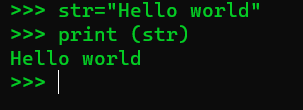
\includegraphics[]{python.png}
		\centering		
		\caption{Comprobar python}
		\label{img:python}
	\end{figure}
	\item Para ejecutar un programa escrito en Python desde la consola  Powershell el comando es el siguiente: 
	\begin{verbatim}
		py HelloWorld.py
	\end{verbatim}
	\item Es posible que la versión de Python, tanto descargada del repositorio oficial como desde Microsoft Store, no tenga el módulo \textit{Serial} (necesario para las comunicaciones con el robot) instalado por defecto. Tan solo es necesario ejecutar en Powershell la siguiente línea de código para instalarlo:
	\begin{verbatim}
		pip install pyserial
	\end{verbatim}
	La ejecución puede verse en la figura \ref{img:pyserial}.
	\begin{figure}[h]
		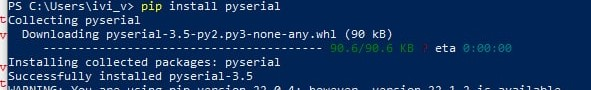
\includegraphics[]{pyserial.jpg}
		\centering		
		\caption{Instalar módulo \textit{Serial} en Python}
		\label{img:pyserial}
	\end{figure}
	\item Para escribir programas en Python puede utilizarse cualquier editor de texto. El mismo instalador de Python instala un IDE propio (en la figura \ref{img:pythonIDE}) suficientemente simple y preparado particularmente para su sintaxis y para ejecutar directamente los programas.
	\begin{figure}[t]
		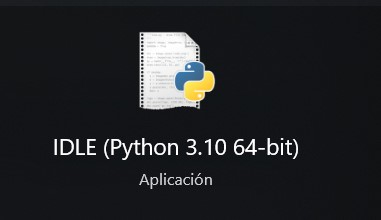
\includegraphics[]{pythonIDE.png}
		\centering		
		\caption{Editor de texto instalado con Python}
		\label{img:pythonIDE}
	\end{figure}
\end{enumerate}
\newpage

